\documentclass[runningheads]{llncs}

%%% Dependencies

%For including github link
\usepackage{hyperref}
% Sets font
\usepackage[T1]{fontenc}

% Include figures, graphs, images, preferably in .eps format
\usepackage{graphicx}

% Clickable links, refs, urls
% Inside the brackets can be removed if cross-references should not be colored
\usepackage[colorlinks=true, allcolors=blue]{hyperref}
\usepackage{color}
\renewcommand\UrlFont{\color{blue}\rmfamily}

% Table lines
\usepackage{booktabs, multirow}

% Matrix dimensions
\usepackage{amsmath} 
\newcommand{\undset}[2]{\underset{\scriptscriptstyle #1}{#2\strut}}

% For todos
\usepackage[colorinlistoftodos]{todonotes}

% Can be used to cite multiple references at once
\usepackage{cite}

% for code snippits
\usepackage{listings}

%%% A lot more dependencies are probably needed, but am tired with looking them all up

\begin{document}

%%% Keep separate sections in own files, and use \input to add them to the main file.
\mainmatter

\title{Document Knowledge Transfer for Aspect-Based Sentiment Classification Using a Left-Center-Right Separated Neural Network with Rotatory Attention}
\author{Emily Fields \and Gonem Lau \and Robbert Rog \and Alexander Sternfeld}
\titlerunning{Document Knowledge Transfer for LCR-Rot-hop++}
\authorrunning{E. Fields, G. Lau, R. Rog, A. Sternfeld}
\institute{Erasmus University of Rotterdam, Burgemeester Oudlaan 50, 3062 PA Rotterdam, the Netherlands\\\email{\{505456ef,500202gl,492751rr,492825as\}@student.eur.nl}}
{\def\addcontentsline#1#2#3{}\maketitle}
\begin{abstract}
Traditional Aspect-Based Sentiment Classification (ABSC) methods make use of domain-specific, costly ontologies to make up for the lack of available aspect-level data. This paper proposes two forms of transfer learning to exploit the plenteous amount of available document data for sentiment classification. Specifically, two forms of document knowledge transfer, pretraining (PRET) and multi-task learning (MULT), are considered in various combinations to extend the state-of-the-art LCR-Rot-hop++ model. For both the SemEval 2015 and 2016 datasets, we find an improvement over the LCR-Rot-hop++ model. Overall, the pure MULT model performs well across both datasets. Additionally, there is an optimal amount of document knowledge that can be injected, after which the performance deteriorates due to the extra focus on the auxiliary task. We observe that with transfer learning and L1 and L2 loss regularisation, the LCR-Rot-hop++ model is able to match or outperform hybrid models that use both ontology and deep learning. Thus, we conclude that transfer learning is a feasible and computationally cheap substitute for the ontology step of hybrid ABSC models.
    \keywords{LCR-Rot-hop++ $\cdot$ Transfer Learning $\cdot$ Pretraining $\cdot$ Multi-Task Learning}
\end{abstract}
% \setcounter{secnumdepth}{5}
\setcounter{tocdepth}{5}

\tableofcontents

\section{Introduction}
% \label{sec:introduction}

% \todo[inline]{Formulation \textit{of the research problem}.

% Motivation: \textit{why actually is the research problem a ‘problem’? Why is our current knowledge of the topic insufficient? Why is further research required?}

% Relevance: \textit{why and for whom is the ‘problem’ important?}}

In the pre-Web era, it was often difficult for companies to gauge the opinions of their large customer bases. While the increasing popularity of the Web provided a virtually inexhaustible source of data, machine learning methods had to be developed for extracting insights from this information. One particularly interesting insight is to extract a sentiment from a segment of text, for example a review. This is what drove the development of Sentiment Analysis in the field of Natural Language Processing (NLP) \cite{Liu2020}. 

This paper specifically considers Aspect-Based Sentiment Analysis (ABSA). ABSA consists of two steps: Aspect Detection (AD) and Aspect-Based Sentiment Classification (ABSC). AD is the task of finding an aspect, such as price, quality, or service of an entity, within a text or review. This paper will focus on ABSC exclusively, which involves determining the sentiment of a given aspect within a given sentence\cite{brauwers2021, Schouten2017}. It is common practice to divide sentiment into three classes: positive, neutral, and negative.

Traditionally, dictionary-based approaches such as that in \cite{Hu2004} have been used, but with the rise of Deep Learning and the ever-increasing computational power of modern machines, a range of new techniques for ABSC have become available. Of the basic ``deep'' models, the Bidirectional Long Short-Term Memory Network (BiLSTM) at first appeared to be the most promising, as illustrated in \cite{Graves2005}. Over the years, however, more sophisticated BiLSTM methods have been developed. One of which is the Left-Center-Right Separated BiLSTM with Rotatory Attention (LCR-Rot) \cite{Zheng2018}, which utilizes separately trained BiLSTM networks for the context to the left of the aspect, the aspect itself, and the context to the right of the aspect, and has been found to outperform previously proposed LSTM-variations \cite{Zheng2018}. Even more recently, the LCR-Rot model has been extended with respect to both the attention mechanism and the word embeddings. Namely, the LCR-Rot-hop model presented in \cite{Wallaart2019} iteratively applies the attention mechanism, while the LCR-Rot-hop++ model proposed in \cite{Trusca2020} builds on this to include hierarchical attention and deep contextual word embeddings. 

Over the past years, a collection of techniques called Transfer Learning (TL) has surged in popularity as a method to improve the performance of machine learning methods. More formally, Transfer Learning involves training a model on auxiliary tasks to improve the performance for our main task. This is particularly interesting when there is few data available for our task at hand. One such method is multi-task learning (MULT), where a model is trained on two tasks simultaneously, as applied in the widely used language model called Bidirectional Encoder Representation from Transformers (BERT) \cite{Devlin2019}. An alternative method is pretraining (PRET), which involves first learning an auxiliary task after which the model is trained for the main task. The latter step is called fine-tuning (FT), meaning a TL model is trained once more on just the main task.

A lack of training data in the same domain as the test data is a persistent issue in machine learning \cite{pan2010}. In ABSC, this is reflected by the limited availability of aspect-level data. As there is more annotated sentiment data available at a document level, i.e. review texts with star ratings, this information can be exploited using TL techniques. \cite{He2018}, for example, showed an improvement in the performance of ABSC in BiLSTMs when PRET and MULT are utilized. We consider four approaches for document knowledge transfer in the LCR-Rot-hop++ model, inspired by \cite{He2018}. The first approach is PRET+FT, in which the model is first pretrained on the document knowledge and then fine-tuned. The second is MULT, where the sentiment of a document and of an aspect are determined simultaneously. While the method proposed in \cite{He2018} does not include a regularization term, we extend the approach by including a regularization term in the loss function as in \cite{Wallaart2019}. The third method is a combination of both PRET and MULT, called PRET+MULT, in which the model is first pretrained at a document level on part of the data, before MULT is applied to the rest of the data. Last, in the fourth and fifth approaches, we develop new methods that incorporate FT into the TL approach, in two models called MULT+FT and PRET+MULT+FT. 

The present work extends the existing literature by implementing document knowledge transfer on the state-of-the-art LCR-Rot-hop++ model, with the aim to further improve its accuracy. Moreover, different L1 and L2 regularisation terms are combined to improve upon the previous works. Additionally, it is analysed how the results for multi-task learning change when the emphasis on the auxiliary task is altered. Last, different sizes of pretraining corpora are used to investigate the effect on the accuracy of our main task. The Python source code of our models can be found at \url{https://github.com/Gogonemnem/seminar-ba-qm}.

The paper continues as follows. First, the related works and their results are discussed in more detail in Sect. 2, after which the data is illustrated in Sect. 3. Subsequently, the methodology is presented in Sect. 4, in which the LCR-Rot-hop++ model and the experimental setup are explained thoroughly. Thereafter, the results are compared with those obtained in the previous literature in Sect. 5. Last, conclusions with the main findings and suggestions for future research are presented in Sect. 6.

% PAST INTRODUCTION

% In the pre-Web era, companies often struggled to gauge the opinions of their large customer bases. Likewise, governments had difficulties in determining the public opinion, which complicated policy-making. The increasing popularity of the Web lead to a virtually inexhaustible source of data, for which manual processing is impossible. Consequently, machine learning methods were developed for extracting information from the data. One of these challenges was to extract a sentiment, either positive, neutral or negative, from a segment of text. The abundance of freely provided opinions is what drove the development of Sentiment Analysis in the field of Natural Language Processing (NLP) \cite{Liu2020}. This paper focuses specifically on Aspect-Based Sentiment Analysis (ABSA), which aims to identify the sentiment towards a given aspect of a product, for example its quality \cite{Schouten2016}.

% ABSA consists of two steps: Aspect Detection (AD) and Aspect-Based Sentiment Classification (ABSC). AD is the task of finding an aspect, such as price, quality, or service of an entity, within a text or review. As illustrated in \cite{Schouten2016}, a wide variety of techniques for AD are available; some focus merely on the frequency of words, whereas others are more complex and exploit machine learning techniques. This paper, however, will focus on ABSC exclusively, hence the models discussed in this work thus focus on determining the sentiment of a given aspect within a given sentence. It is common practice to divide sentiment into three classes: positive, neutral, and negative.

% Traditionally, dictionary-based approaches such as that in \cite{Hu2004} have been used, but with the rise of Deep Learning methods and the ever-increasing computational power of modern machines, a range of new techniques for ABSC have become available. Of the basic "deep" models, the Bidirectional Long Short-Term Memory Network (BiLSTM) at first appeared to be the most promising, as illustrated in \cite{Graves2005}. Over the years, however, more sophisticated BiLSTM methods have been developed, one of which is the Left-Center-Right Separated BiLSTM with Rotatory Attention (LCR-Rot) \cite{Zheng2018}. This model utilizes separately trained BiLSTM networks for the context to the left of the aspect, the aspect itself, and the context to the right of the aspect, and has been found to outperform previously proposed LSTM-variations \cite{Zheng2018}. Even more recently, the LCR-Rot model has been extended with respect to both the attention mechanism and the word embeddings. Namely, the LCR-Rot-hop model presented in \cite{Wallaart2019} iteratively applies the attention mechanism, while the LCR-Rot-hop++ model proposed in \cite{Trusca2020} builds on this to include hierarchical attention and deep contextual word embeddings. 

% Over the past years, a collection of techniques called Transfer Learning has surged in popularity due to its effectiveness. More formally, Transfer Learning is the idea to train a model on auxiliary tasks to improve the performance for our main task. The widely used language model, Bidirectional Encoder Representation from Transformers (BERT) \cite{Devlin2019}, is trained on two tasks simultaneously, which is called multi-task learning (MULT). Learning two semantically related tasks can provide positive external effects in their performance as it leads to shared layers within the model. Instead of learning them at the same time, one could also first learn the auxiliary task before learning the main task, which is referred to as pretraining (PRET). After the PRET and/or MULT phases are finished, a model can be trained on our main task specifically, which is called fine-tuning (FT).

% A persistent issue of ABSC is the limited availability of data on such a specific aspect-level. More generally, the lack of training data in the same domain as the test data is a common issue in machine learning problems \cite{pan2010}. Recently, the idea of document knowledge transfer has been popularized by \cite{He2018}, which showed an improvement in the performance of aspect-level sentiment analysis in BiLSTMs. As there is more annotated sentiment data available at a document level, one can exploit this information using Transfer Learning techniques\todo{I still think he wants more discussion of transfer learning in general here, based on what he said in the meeting}. The present work extends the existing literature by implementing document knowledge transfer on the LCR-Rot-hop++ model, with the aim to improve its accuracy even further. More specifically, four approaches for document knowledge transfer will be considered. The first approach is known as pretraining, where the LCR-Rot-hop++ model is first pretrained on the document knowledge, with the idea that the model learns sentiment on a higher document-level. The second method for document knowledge transfer is multi-task learning, where the sentiment of a document and of an aspect are determined simultaneously. The third approach combines both methods: the model is first pretrained at a document level, before multi-task learning is applied. Last, in a fourth approach, a new transfer learning method is tested which combines pretraining, multi-task learning, and fine-tuning.

% This paper contributes to the existing literature in three ways. First, document knowledge transfer is applied to the state-of-the-art LCR-Rot-hop++ model. Secondly, fine-tuning is incorporated into the transfer learning approach, which has not been done in this setting. Finally, we regularize the loss function to avoid overfitting.

% The paper continues as follows. First, the related works and their results are discussed in more detail in Sect. 2, after which the data is illustrated in Sect. 3. Subsequently, the methodology is presented in Sect. 4, in which the LCR-Rot-hop++ model and the experimental setup are explained thoroughly. Thereafter, the results are compared with ones obtained in the previous literature for the same dataset in Sect. 5. Finally, a conclusion of the main findings and a discussion containing directions for future research are presented in Sect. 6.
\section{Related Work}
\label{sec:literature}
This section discusses the literature related to our research. Methods for addressing ABSC are classified into three types: knowledge-based methods, machine learning methods, and hybrid approaches \cite{brauwers2021}. The most important findings for key methods within these categories are discussed, building up to a brief summary of LCR-Rot-hop++. Last, results of previous works using document knowledge transfer are analysed.

\subsection{ABSC Models}

Traditionally, dictionary-based approaches have represented the foundation for ABSC. One of the first implementations of such an approach was presented in \cite{Hu2004}. In this method, a basic collection of words is manually labeled. Next, a synonym/antonym graph is used, to further classify words. To illustrate, a synonym of a word with a positive sentiment will be labeled positive as well.

Dictionary-based approaches are, however, manually intensive, which has led to an increase in the popularity of machine learning for ABSC. BiLSTMs, specifically, form the basis of many advanced models for ABSC. More precisely, over the years, extensions of BiLSTMs have been developed to better account for the context surrounding the aspect. One of the more popular such extensions is LCR-Rot, which utilizes left-center-right separated LSTMs as well as a rotatory attention mechanism to create separate target representations for the aspect itself, the context to the left, and the context to the right \cite{Zheng2018}. After that, the model applies a classification head over the concatenation of their representations, and has been found to outperform several other machine learning models \cite{Zheng2018}. 

% The first such approaches involved standard algorithms such as Na\"{\i}ve Bayes, Maximum Entropy classification, and Support Vector Machines were popular \cite{Pang2002}, but more recently, neural networks have been applied to the field of NLP \cite{Do2019}. Some examples are Convoluted Neural Networks (CNNs), which have been shown to be successful in many NLP tasks, including ABSC \cite{Kim2014}, as well as Recurrent Neural Networks (RNNs), which utilise hidden states to capture context dependencies. These methods, however, suffer from the vanishing gradient problem, leading to short-term memory, which drove the development and use of LSTMs \cite{Hochreiter1997}. 

The LCR-Rot model has been further extended in many directions, most notably with respect to the attention mechanism and the word embeddings. In particular, \cite{Wallaart2019} proposes an LCR-Rot-hop model that iteratively applies the rotatory attention mechanism proposed in \cite{Zheng2018}, which outperforms the base model as it can better capture sentiment presented in a complex sentence. In \cite{Trusca2020}, the LCR-Rot-hop++ model is proposed as a further extension of this, by using a hierarchical attention mechanism and deep contextual word embeddings. The advantage of using hierarchical attention is that the relevance of the attention vectors is calculated also at a sentence level next to the word-level attention. Deep contextual word embeddings are useful in that they take into account the context of words and thus can better handle the semantics of a sentence. These two additions to the LCR-Rot-hop model have been shown to increase prediction accuracy for two standard datasets \cite{SemEval2015, SemEval2016}. 

Dictionary-based approaches and machine learning models are often combined into hybrid models for ABSC. Two-step classification methods have been proven to be particularly effective compared to combined models  \cite{Cambria2018,Chikersal2015,Schouten2016,Schouten2017,Wallaart2019}. One of the first two-step approaches was proposed in \cite{Chikersal2015}, and improvements on this method are proposed in a sequence of works \cite{Schouten2016,Schouten2017,Wallaart2019} followed by \cite{Trusca2020}. \cite{Trusca2020} presents HAABSA++, where a domain ontology is used to determine the sentiment for each sentence and LCR-Rot-hop++ is applied to any sentences for which the ontology is inconclusive, also leading to better performance than solely using LCR-Rot-hop++.

\subsection{Document Knowledge Transfer} 

The performance of the LCR-Rot-hop++ model depends on the scale of the available training data, as limited training data can lead to a lower accuracy. Ideally, one would use aspect-level data, as the model is used for sentiment analysis at the aspect level. However, the availability of annotated aspect-level data is limited \cite{pan2010, He2018}. To illustrate, both \cite{Trusca2020} and \cite{Wallaart2019} use the standard SemEval 2015 and SemEval 2016 datasets \cite{SemEval2015, SemEval2016}, which are relatively small. Due to the limited availability of aspect-level data, the LCR-Rot-hop++ model may not reach its full potential. To overcome this issue, one can consider coarser data, such as document level or sentence level data. There is an abundance of this type of data, for instance Yelp reviews \cite{Tang2015}. 

Document knowledge transfer can be motivated from three perspectives: human learning, pedagogy, and machine learning \cite{Ruder2019}. From the point of view of human learning, it is clear that we frequently use knowledge acquired from learning related tasks when learning a new task. Equally, from a pedagogical perspective, we often learn the foundations first, before using this knowledge to learn more complex skills. Last, document knowledge transfer improves generalization by introducing an inductive bias, which creates a preference for hypotheses that explain more than one task \cite{Caruana1993}. In this paper, we investigate which method for document transfer knowledge performs best, specifically, we consider combinations of pretraining (PRET), multi-task learning (MULT), and fine-tuning (FT). 

\subsubsection{PRET.}
Pretraining is the act of training a model on a task semantically related to your target task, prior to training for your target task \cite{Ruder2019, He2018}. This technique has shown great success in language models such as BERT in \cite{Devlin2019}. BERT was trained to perform two tasks which helped the model understand language, after which it can be fine-tuned for a wider variety of language tasks. As shown in \cite{He2018}, pretraining a BiLSTM on document-level data improved the results obtained on an aspect level. 

\subsubsection{MULT.}
In contrast to PRET, when using MULT the model is trained for the target task and the semantically related task simultaneously \cite{Ruder2019}. The purpose of this is to improve generalization, which might lead to more effective knowledge transfer. For example, \cite{Subramanian2018} demonstrated that multi-task learning is able to produce good word embeddings.

\subsubsection{FT.}
In PRET and MULT, one uses the semantically-related task to improve performance on the target task. With FT, one only trains on the target task. Therefore, it is necessary in combination with PRET, but optional with MULT. To illustrate, the BERT language model first gets trained using a MULT approach on general language tasks, after which it can be trained for specific tasks using an FT approach \cite{Devlin2019}.

% Three types of methods are classified for addressing ABSA: knowledge-based methods, machine learning methods, and a hybrid approach \cite{schouten_survey_2016}. Earlier methods exploit (implicit) rules in human language. For example, aspects were detected by its frequency \todo{citation needed}. Some extracted sentiment by assigning scores to words in the dictionary \todo{citation needed}. While others exploited syntax rules such as adjectives usually being close to nouns \todo{citation needed} and negations \todo{citation needed}. However, some drawbacks of these methods are the dependence on linguistic correctness \todo{citation needed} and the manual labor required to implement these rules \cite{bielikova_hybrid_2020}. 

% Therefore, machine learning methods were investigated. Early successful models include Maximum Entropy, Conditional Random Field, and Support Vector Machine methods \todo{citations needed}. These were further developed to incorporate neural models such as GRU \todo{this one im not 100\% sure about} and Long Short-Term Memory models \todo{maybe other methods are better suited}. While these methods are quite efficient and more robust to linguistic errors, they still require manual labor to label the large training dataset. Furthermore, results might differ across domains\todo{citation needed}. For example, a hot environment might be preferable in a spa resort but not for a ski resort.

% It turns out that combining both approaches sequentially further improved results, developing into the two-step Hybrid Approach for Aspect-Based Sentiment Analysis \todo{citation needed}. The first step is to determine the sentiment using domain ontology \todo{citation needed, also is domain ontology general? bc i do not mention LCR next}. The second step gathers all inconclusive sentiments and employs machine learning techniques to determine sentiment.

% \todo[inline]{Other direction of improving HAABSA: document knowledge transfer (adds document level sentiment analysis)}

% Another method to improve performance is to incorporate document-level sentiment analysis \cite{he_exploiting_2018}. Knowledge from a lower level is added and is less laborious to obtain, meaning that less aspect-level data is needed. \todo{talk about PRET, MULT and PRET+MULT}

% \todo[inline]{Combine both advancements}

% We explore the advancements of \cite{bielikova_hybrid_2020, he_exploiting_2018}, by combining both lines of thought. Our hypothesis is that document knowledge transfer will improve the performance of the advanced neural network.
\section{Data}
\label{sec:data}

% \todo[inline]{Data: \textit{What kind of data are you going to use? If the data is available already: what are the key data characteristics?}}

% \todo[inline]{SemEval 2015 and/or SemEval 2016, and find source for document level data (He used Yelp2014 and Amazon Electronics dataset). Remove implicit data. Maybe some key characteristics are useful: Total count, Number of positives/negatives? Show whether the data is balanced or not, important for training an ML model}

The datasets used for ABSC are the SemEval 2015 \cite{SemEval2015} and SemEval 2016 data sets \cite{SemEval2016}. Specifically, our analysis focuses on restaurant reviews. Each review consists of one or more sentences, and each sentence contains the sentiment on one or more aspects. The sentiment can either be positive, neutral, or negative. In our research we focus on explicit aspects, which means that the aspect is present in the sentence. Figure \ref{fig:xml} shows an example sentence from the SemEval 2016 dataset in the XML markup language. This example shows that, in a review, multiple aspects can be present and the sentiment towards different aspects may differ. Table \ref{describeData} gives the descriptive statistics of the SemEval 2015 and the SemEval 2016 data sets. One can notice that there are relatively few neutral reviews. Furthermore, in most data the positive class is the majority class, except for the test data of the SemEval 2015 data set. The 2015 dataset is noticably smaller than the one from 2016.


\begin{figure}
    \centering
    \frame{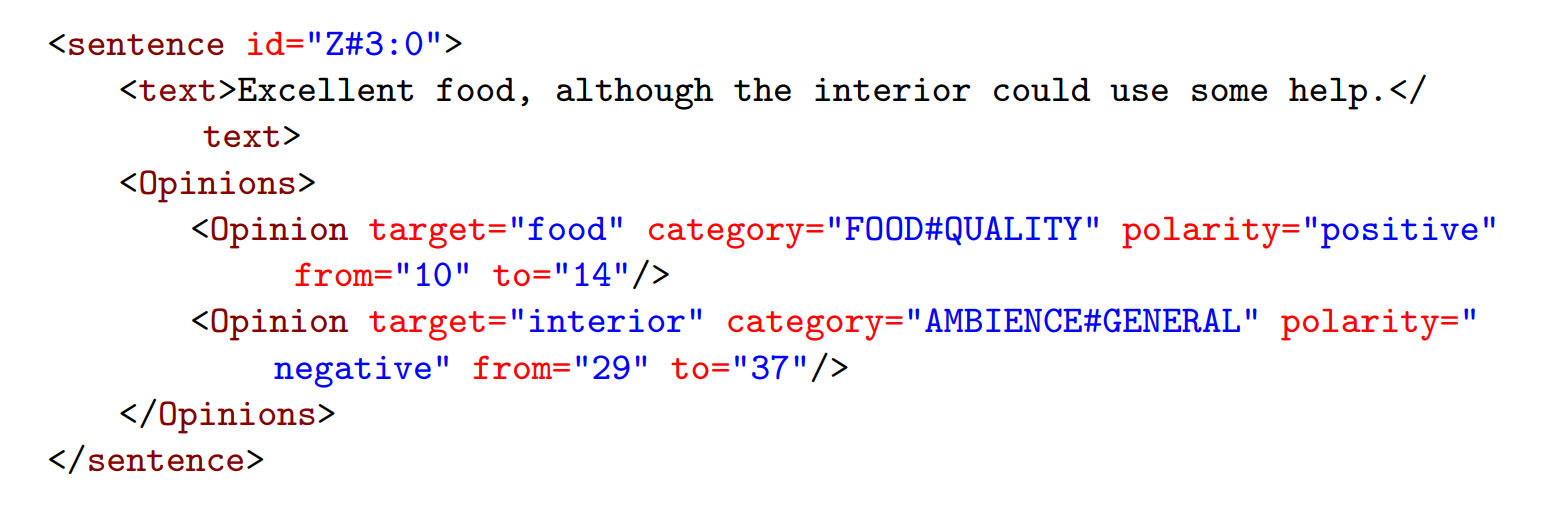
\includegraphics[scale = 0.4]{Images/xml code.PNG}}
    \caption{A sentence from the SemEval 2016 dataset.}
    \label{fig:xml}
\end{figure}


We use a document-level dataset from Yelp2014 \cite{Tang2016} for pretraining, as it matches the domain of our aspect-level data: restaurants. However, these reviews are classified on a 5-point scale. Therefore, the reviews will be labeled in the following way: reviews with ratings $>3$, $=3$, and $<3$ are labeled as positive, neutral, and negative, respectively. Similar to \cite{He2018}, a balanced sample of 30000 will be extracted from the dataset to obtain our pretraining corpus. As Table \ref{describeData} shows, there is a significant lack of neutral examples in the aspect-level data. Therefore, the balancing of the pretraining corpus allows the model to see an ample amount of documents for each category. To make our data suitable for multi-task learning, each aspect-level datapoint is paired with a random document from our sample. As there are many more documents available than aspects, we upsample our aspect-level data with a factor of three. This value was chosen from intuition, as too little upsampling will not allow us to exploit many documents whereas too much upsampling will likely lead the model to overfit due to the duplicates in the aspect data.

\begin{table}[h]
\caption{Descriptive statistics of the SemEval 2015 and semEval 2016 datasets, split into training and test data.}
\label{describeData}
\setlength{\tabcolsep}{8.2pt}
\begin{tabular}{@{}lccccccc@{}}
\toprule
\multicolumn{1}{c}{\multirow{2}{*}{Dataset}} & \multicolumn{2}{c}{Positive} & \multicolumn{2}{c}{Neutral} & \multicolumn{2}{c}{Negative} & Total \\ \cmidrule(l){2-8} 
\multicolumn{1}{c}{}                         & Freq          & \%           & Freq          & \%          & Freq          & \%           & Freq  \\ \midrule
SemEval-2015 training data                   & 963           & 75.3         & 36            & 2.8         & 280           & 21.9         & 1279  \\
SemEval-2015 test data                       & 208           & 34.7         & 38            & 6.3         & 354           & 59.0         & 600   \\
SemEval-2016 training data                   & 1321          & 70.1         & 73            & 3.9         & 490           & 26.0         & 1884  \\
SemEval-2016 test data                       & 487           & 74.4         & 32            & 4.9         & 136           & 20.8         & 655   \\ \bottomrule
\end{tabular}
\vspace{-5mm}
\end{table}

\section{Methodology}
\label{sec:methodology}
This section discusses the methodology used to obtain the results. First, the LCR-Rot-hop++ model is explained in detail. Thereafter, the four methods for document knowledge transfer (PRET, MULT, PRET+MULT, and PRET+MULT+FT) are elaborated upon. Last, the experimental setup for obtaining the results is given.
% \todo[inline]{Methodology: \textit{what kind of econometric methods and statistical techniques are you going to use to investigate the research problem? Why are those techniques suitable to address your research question(s)?}}

\subsection{LCR-Rot-hop++}

In this section we present the LCR-Rot-hop++ model \cite{Trusca2020}. This model is an extension of the LCR-Rot-hop model \cite{Wallaart2019}, and is consideed a state-of-the-art model for ABSC.

The BERT model is used to generate deep contextual word embeddings. The final representation of a word is calculated by summing its last four hidden states. We follow the approach of \cite{Trusca2020} in that we use the BERT-Base model with $L=12$ layers, $A=12$ attention heads, and $H=768$ hidden units. Each sentence is divided into the left context, the aspect (target), and the right context. The BERT word embeddings are divided accordingly into three embedding matrices, $S^l = [s_1^l,...,s_L^l]$, $S^t = [s_1^t,...,s_T^t]$, and $S^r = [s_1^r,...,s_R^r]$, where $s_i^j$ is the embedding for word $i$ in part $j$. Each embedding matrix is fed through the corresponding BiLSTM. This results in the hidden states, denoted as $H^l = [h_1^l,...,h_L^l]$, $H^t = [h_1^t,...,h_T^t]$, and $H^r = [h_1^r,...,h_R^r]$. The size of $h_i^j$ is a hyperparameter to be optimized, which we denote as the dimension $d$. 

Subsequently, the output from the left, center, and right BiLSTM are iteratively propagated through a rotatory attention mechanism. This iterative mechanism consists of two steps: Target2Context and Context2Target. The prior is used to obtain a representation from the context by focusing on specific words that are related to the target, hence, Target2Context. Afterward, this new context representation is used to acquire a better representation of the target itself, hence Context2Target. The newly obtained target representations in step 2 can be used to execute step 1, leading to an iterative process. Both steps are now explained in more detail.

\subsubsection{Step 1: Target2Context Attention Mechanism.}
First, an average target representation $r^{t_p}$ is computed using an average pooling layer over the vectors in $H^t$. Then, for both the left and the right context, an attention function $f$ is computed for each word to determine the level of focus. This attention function is defined as
\begin{equation}
    \undset{1\times 1}{f(h_i^l, r^{t_p})}=\mathrm{tanh}(\undset{1\times 2d}{h_i^{l'}}\times \undset{2d\times 2d}{W_c^l}\times \undset{2d\times 1}{r^{t_p}}+\undset{1\times 1}{b_c^l}),
\end{equation}
where $W_c^l$ is a weight matrix and $b_c^l$ is a bias. Next, these attention scores are normalized by applying the softmax function
\begin{equation}
    \alpha_i^l=\frac{\mathrm{exp}(f(h_i^l,r^{t_p}))}{\sum^L_{j=1} exp(f(h_j^l,r^{t_p}))}.
\end{equation}
Last, the left and right context are represented in a single vector by summing the weighted hidden states of the embedding matrix as follows
\begin{equation}
    \undset{2d\times 1}{r^l}=\sum^L_{i=1} \undset{1\times 1}{\alpha_i^l}\times \undset{2d\times 1}{h_i^l}.
\end{equation}
We compute $r^r$ in a similar fashion as $r^l$.

\subsubsection{Step 2. Context2Target Attention Mechanism.}
In the second step, we generate new target representations in a similar way, following the previous three equations, with the exception that we use $r^l$ and $r^r$ in place of $r^{t_p}$. This leads to two new target representations: one based on the left context and one based on the right context. The following equation denotes the left Context2Target representation
\begin{equation}
    \undset{2d\times 1}{r^{t_l}}=\sum_{i=1}^T \undset{1\times 1}{\alpha_i^{t_l}}\times \undset{2d\times 1}{h_i^t}.
\end{equation}
We again obtain the right Context2Target representation $r^{t_r}$ similarly as $r^{t_l}$.

In \cite{Wallaart2019}, the attention mechanism is improved by iteratively applying the steps. The newly obtained target representations in step 2 can be utilised to generate new attention scores in step 1. This extends the LCR-Rot model to the LCR-Rot-hop model, as each iteration of the attention mechanism is called a ``hop''. This is further improved in \cite{Trusca2020} by applying a hierarchical attention mechanism, the architecture of which is shown in Fig.  \ref{fig:haabsa++}.
\begin{figure}[h!]
    \centering
    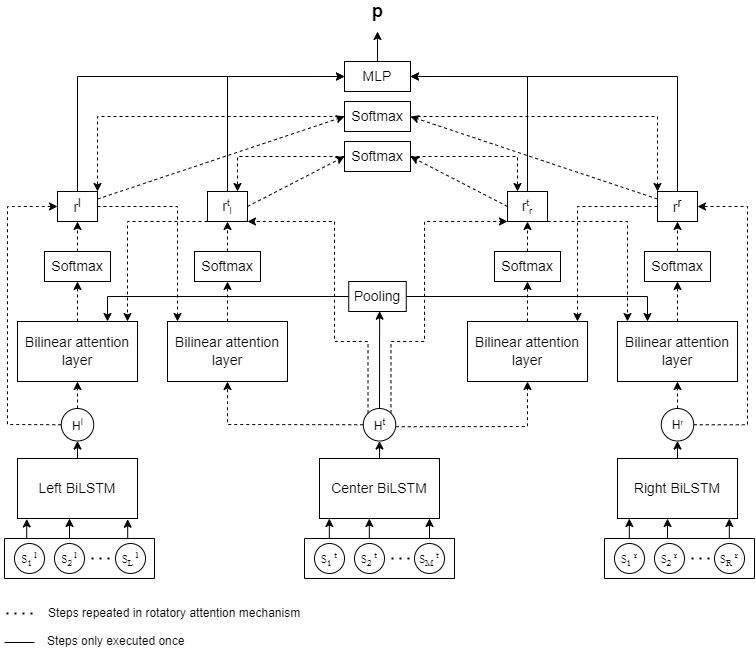
\includegraphics[width=\textwidth]{Images/LCR-Rot-Hop++.jpg}
    \caption{LCR-Rot-hop++ model}
    \label{fig:haabsa++}
\end{figure}

Hierarchical attention consists of scaling the Context\-2\-Target and Target\-2\-Context vectors using a sentence-level relevance score. Intuitively, the hierarchical attention decides whether more emphasis should be put on the left or right context. 
First, an attention function $f$ is computed, which is defined as
\begin{equation}
    \undset{1\times 1}{f(v^i)}=\mathrm{tanh}(\undset{1\times 2d}{v^{i'}}\times \undset{2d\times 1}{W}+\undset{1\times 1}{b}),
\end{equation}
where $v^i\in \{r^l, r^{t_l}, r^{t_r}, r^r\}$ is representation $i$ of the input sentence, $W$ is a weight matrix, and $b$ is a bias term. Then we compute new attention scores for each pair $\{r^l,r^r\}$ and $\{r^{t_l},r^{t_r}\}$ separately. The attention scores and newly obtained representations are defined as
\begin{equation}
    \alpha^i=\frac{\mathrm{exp}(f(v^i))}{\sum_{j=1}^2 \mathrm{exp}(f(v^j))},
\end{equation}
\begin{equation}
    \undset{2d\times 1}{v^i}=\undset{1\times 1}{\alpha^i}\times \undset{2d\times 1}{v^i}.
\end{equation}
As in \cite{Trusca2020}, we apply the attention weighting separately in each iteration of the rotatory attention mechanism, both on the pairs of intermediate context vectors and on the pairs of target vectors. In other words, after each Target2Context step, the hierarichal attention is applied to the $\{r^l,r^r\}$ pair, while after each Context2Target step, the hierarichal attention is applied to the $\{r^{t_l},r^{t_r}\}$ pair.

\subsection{Knowledge Transfer}
This paper considers several different approaches for document knowledge transfer. Each approach consists of one or more of the following building blocks: PRET, MULT, and FT. In this section, each building block will be described separately. Furthermore, Fig. \ref{fig:pretmultft} displays which compositions of PRET, MULT and FT are implemented in this paper. In the notation of each building block, we consider the two tasks $\tau_1$ and $\tau_2$. Let $\tau_2$ be our task of interest, namely ABSC. In contrast, $\tau_1$ is sentiment classification at a document level, which is semantically related to our main task. Therefore, teaching our model to execute $\tau_1$ will enlighten it with knowledge that can be used for better executing $\tau_2$. 

\begin{figure}[h!!!!!]
    \centering
    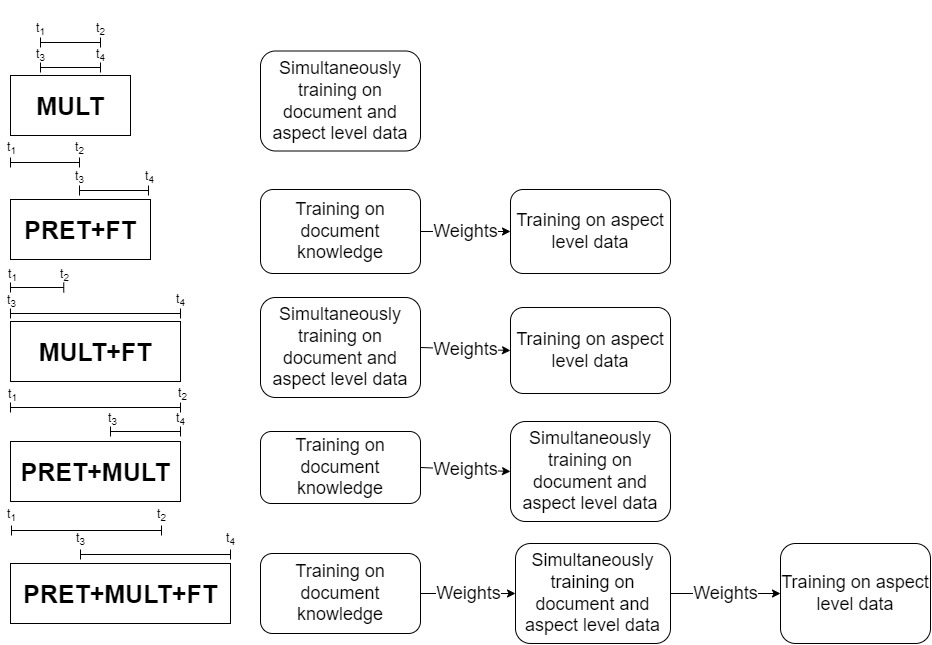
\includegraphics[width=\textwidth]{Images/PRET_MULT.jpg}
    \caption{An overview of the different document knowledge transfer approaches. The target task is executed in the time interval $[t_3, t_4]$, whereas the semantically related task is executed in the time interval $[t_1, t_2]$}
    \label{fig:pretmultft}
\end{figure}

\subsubsection{PRET.}
In the pretraining stage only $\tau_1$ is executed, which trains the model for sentiment analysis at a document level. Specifically, the documents are put through the left, center, and right BiLSTM, after which the final hidden layers of all words are pooled. The pooled hidden layers of the three BiLSTMs are concatenated and fed into a classification layer. The aim of this stage is to pretrain the BiLSTMs, as it is expected that the BiLSTM weights obtained in the PRET stage transfer the information from the document level sentiment classification to improve the accuracy at the aspect level.

\subsubsection{MULT.}
During the multi-task stage, tasks $\tau_1$ and $\tau_2$ are executed simultaneously.  In this approach, the three BiLSTMs are trained simultaneously on the document-level data and on their corresponding part of the aspect-level data (left, target, or right). Each aspect-level data point is paired to a document-level data point. Thus, the embedding layer and the three BiLSTMs in the LCR-Rot-hop++ model are shared for $\tau_1$ and $\tau_2$. The document-level data is processed the same as in the PRET stage. For the aspect-level data, the outputs from the BiLSTMs are directed to the corresponding attention mechanism, which finally leads to probabilities regarding the aspect-based sentiment.

% The data for $\tau_1$ can be propagated through both the left, right, and/or center BiLSTM of the LCR-Rot-hop++ model. After the BiLSTM outputs a document representation, it will be sent to a separate classification layer. In the end, the embedding layer and a number of the three BiLSTMs in the LCR-Rot-hop++ will be shared for $\tau_1$ and $\tau_2$. Table \ref{tab:MULT ways} shows the combinations which will be tested. 

% Please add the following required packages to your document preamble:
% \usepackage{booktabs}
%\begin{table}[htbp]
%\caption{}
%\label{tab:MULT ways}
%\begin{tabular}{@{}l@{}}
%\toprule
%\textbf{LSTM used for document sentiment %classification} \\ \midrule
%Left LSTM + right LSTM + center LSTM                     \\
%Left LSTM + right LSTM                                   \\
%Left LSTM                                                \\
%Right LSTM                                               \\ \bottomrule
%\end{tabular}
%\end{table}

The parameters are set by minimizing the loss function below.

\begin{equation}
    L = J + \lambda U + \omega \|\Theta\|_1 + \Omega  {\|\Theta\|_2}^2
\end{equation}
In this loss function, $J$ is the mean loss per training batch corresponding to our primary task $\tau_2$. Likewise, $U$ is the mean loss per training batch corresponding to our secondary task $\tau_1$. The loss $U$ is weighted with a parameter $\lambda \in (0,1)$, which can be interpreted as the importance of $\tau_1$ for performing $\tau_2$. Last, $\omega$ and $\Omega$ denote the weights of the L1 and L2 regularisation terms, respectively. The L1 regularisation considers the absolute value of the coefficients, whereas the L2 regularisation considers the squared coefficients. 

\subsubsection{FT.}
The fine-tuning stage can be used as the final stage for training a model. In the FT stage, only $\tau_2$ is executed. In this context, this means that only ABSC is performed. The goal of this stage is to tweak the model, such that it performs best for the target task. Whereas previous stages have taught the model more general knowledge, the FT stage aims at preparing the model solely for the target task.

\subsection{Experimental Setup}
To verify the added value of the TL approaches, we test all combinations as presented in Sect. 4.2 and compare their performance without document knowledge transfer. The following section describes in more detail how we find the best models for each combination.

\subsubsection{Hyperparameter Tuning.}

Hyperband is used to find the optimal hyperparameters \cite{Li2018}. As hypertuning all models over all stages is computationally infeasible, a heuristic  will be used for setting the hyperparameters. Namely, for each dataset, the optimal hyperparameters for the MULT model and the FT model are computed. These hyperparameters will be generalized over all building blocks of the model. Models which use hyperparameters from the tuned FT model are referred to as FT-based models. Models which use hyperparameters from the tuned MULT model are referred to as MULT-based models. Thus, each approach in Fig. 2 is executed using both the FT hyperparameters and the MULT hyperparameters. For the FT-based PRET+MULT+FT model, $\lambda$ has not been optimised in the hypertuning. Hence, the $\lambda$ from MULT tuning will be generalised to this model as well. Note that we do not run an FT-based model for MULT nor PRET+MULT, nor a MULT-based model for PRET+FT, as these parameter and TL approach combinations are likely to be suboptimal. 

\subsubsection{Model Training.}
Early stopping is applied to determine the number of training epochs with different levels of patience for the stages. This means that when the performance on the validation set has not increased during the patience epochs, the epochs after the current best epoch, training is stopped and the optimal model weights are restored. For the PRET stage, the performance measure is the validation loss (categorical cross-entropy). The PRET corpus is large compared to the aspect level data, so for computational efficiency a relatively low patience of 3 is chosen here. Similarly, for the MULT stage, we use early stopping with respect to the combined validation loss described in (8). We allow a higher patience of 10 as the per epoch time is considerably lower, making it more affordable. Last, for the FT stage, early stopping is done with respect to the validation accuracy, as this is our measure of interest. Again, a patience of 10 will be used. The loss functions in all stages, including the benchmark LCR-Rot-hop++, are regularised to prevent overfitting. Both L1 and L2 regularisation are used, the weights of which are optimised by the aforementioned hyperband for both FT-based and MULT-based models.

\subsubsection{Model Evaluation.}

We evaluate the various approaches using the out-of-sample accuracy measure. This measure allows us to see, after training, how often a model correctly predicts the sentiment of an aspect. We note that this measure weights the performance for each sentiment class according to how many observations there are for each sentiment, meaning it does not heavily penalise poor performance in a small sentiment class. As we observe in our data that there are very few neutral observations compared to positive and negative observations, we acknowledge that poor model performance when predicting a neutral sentiment might not be strongly reflected in the accuracy. For this reason, we also evaluate the models using a confusion matrix, to identify in which cases the model wrongly predicts the sentiment. A confusion matrix displays the predicted sentiment class and the corresponding observed sentiment class.

\subsubsection{Sensitivity Analysis.}

To analyse how sensitive the models are to both TL approaches, a sensitivity analysis is performed. First, PRET will be investigated; in particular, we will look at the effect of the size of the pretraining corpus on the model accuracy. Pretraining documents will be added in steps of 3000 up until 30000, our initial corpus. It could be that adding too many documents will lead to the model overfitting on our auxiliary task, whereas using too few documents might leave the model's knowledge lacking.

Additionally, the effect of the level of emphasis on the auxiliary task in MULT will be inspected. Mathematically, this means that we will increase $\lambda$ in (8) with steps of 0.1, starting at 0.1 up until 0.95. Higher values of $\lambda$ put a higher emphasis on the auxiliary task, whereas lower values deem the document classification of less importance. 
\section{Results}
In this section, the performance of the various document knowledge transfer approaches in the LCR-Rot-hop++ model is analysed. First, the accuracy of each model is analysed, before we examine the confusion matrix of the best performing model compared to the benchmark, to consider the performance per sentiment. Last, in a sensitivity analysis it is shown how the performance is affected by changes in $\lambda$. The  hyperparameters for each of the models can be found in Table \ref{tab:hyperparams} in the appendix.

%In the following subsection, the results of several sensitivity analyses are presented, to show how the performance is affected by changes in $\lambda$ and in the size of the pretraining corpora. The  hyperparameters for each of the models can be found in Table \ref{tab:hyperparams} in the appendix.

\subsection{Model Performance}

Table \ref{tab:resultsModel} shows the results of the benchmark LCR-Rot-hop++ model with different hyperparameters and different combinations of document knowledge transfer approaches, for the data of SemEval 2015 and SemEval 2016. All losses, including that of the benchmark LCR-Rot-hop++ model without document knowledge transfer, are regularised using the L1 and L2 regularisation terms, allowing for a fair comparison. We find that several TL models outperform the benchmark LCR-Rot-hop++ model, for both datasets, suggesting there is added value in incorporating document knowledge transfer in the base model.

\begin{table}[h]
\caption{Results of LCR-Rot-hop++ with various forms of document knowledge transfer, alongside the benchmark model without document knowledge transfer, for the SemEval 2015 and SemEval 2016 datasets.}
\label{tab:resultsModel}
\setlength{\tabcolsep}{38pt}
\begin{tabular}{@{}lcc@{}}
\toprule
\multicolumn{1}{c}{\multirow{2}{*}{Settings}} & \multicolumn{2}{c}{Accuracy} \\ \cmidrule(l){2-3} 
\multicolumn{1}{c}{}                          & SemEval 2015  & SemEval 2016 \\ \midrule
\textit{Benchmark model}                      &               &              \\
LCR-Rot-hop++                                 & 79.5\%        & 88.1\%       \\ \midrule
\textit{FT-based models}                      &               &              \\
MULT+FT                                       & 79.7\%        & 88.3\%       \\
PRET+FT                                       & 80.5\%        & 88.6\%       \\
PRET+MULT+FT                                  & 79.8\%         & 88.4\%       \\ \midrule
\textit{MULT-based models}                    &               &              \\
MULT                                          & 81.7\%        & 88.5\%       \\
MULT+FT                                       & 79.2\%        & 88.4\%       \\
PRET+MULT                                     & 81.2\%        & 88.2\%       \\
PRET+MULT+FT                                  & 81.3\%        & 88.2\%       \\ \bottomrule
\end{tabular}
\footnotesize\textit{Note}. The FT-based models are constructed using the optimal hyperparameters from a model with only the FT stage, as is the LCR-Rot-hop++ benchmark model. The MULT-based models use the optimal hyperparameters for a pure MULT model.
\vspace{-3mm}
\end{table}
For the SemEval 2015 dataset, all models with TL outperform the benchmark model, with the exception of the MULT-based MULT+FT. The largest improvement in accuracy, 2.2 percentage points, is observed for the MULT model. Similarly, for the SemEval 2016 dataset, we observe that all TL models outperform the benchmark. Here, the biggest improvements are observed for the PRET+FT and MULT models, which exceed the accuracy of the benchmark model by 0.5 and 0.4 percentage points, respectively. The differences in performance for this dataset are smaller, likely because it is larger and more balanced. Given that transfer learning aims to handle limited data availability and data imbalance by supplying the model with additional examples of a similar task, it is indeed to be expected that these approaches have greater impact in the 2015 dataset. 

Based on the accuracy measures, we conclude that the analysed TL models show potential to boost the accuracy of the existing LCR-Rot-hop++ model. Overall, the MULT model performs best, as it leads to the greatest improvements in accuracy across the two datasets. In comparison to the existing state-of-the-art HAABSA++ model, we observe that our MULT model outperforms HAABSA++ for the SemEval 2016 dataset, by 1.5 percentage points, and matches its performance for the SemEval 2015 dataset, at 81.7\% accuracy. 

One plausible reason for MULT outperforming PRET approaches is catastrophic forgetting \cite{Chen2020}. Knowledge learned in the PRET stage might be forgotten when the model is retrained on the main task. In MULT, the main and auxiliary task are learned simultaneously, making the document knowledge more recent and prevalent. As shown in \cite{Chen2020}, multi-task learning provides a solution to catastrophic forgetting.

%We note that the HAABSA++ model does not include the L1 and L2 regularisation terms, so we cannot entirely attribute the increased performance for the 2016 data to our TL approach, and there might also have been slight computational differences, for example with the searched range for hyperparameter tuning, which could explain the differences in the results. Still, we conclude that our model demonstrates comparable performance to HAABSA++ across the two basic datasets. 

\subsection{Model Performance per Sentiment Class}
Next, we compare the confusion matrices of the LCR-Rot-hop++ benchmark model and the MULT model. This comparison allows us to further investigate how the classifications differ per sentiment. The SemEval 2015 data will be used as this is where the greatest differences are expected, as explained in the previous section. We also consider the confusion matrix for the PRET+FT model, as it showed a slight improvement over the MULT model for the SemEval 2016 dataset. As the confusion matrices for the MULT and PRET+FT models show similar results, the PRET+FT confusion matrix is displayed in Table \ref{tab:confusion matrix:pret} in the appendix. 
\begin{table}[h]
\caption{Confusion matrix of the benchmark LCR-Rot-hop++ model for the SemEval 2015 data.}
\label{tab:confusion matrix LCR}
\setlength{\tabcolsep}{28.3pt}
\begin{tabular}{@{}lccc@{}}
\toprule
                   & \multicolumn{3}{c}{Predicted sentiment} \\ \midrule
Observed sentiment & Negative     & Neutral    & Positive    \\ \midrule
Negative           & 179          & 0          & 29          \\
Neutral            & 20           & 0          & 18          \\
Positive           & 56           & 0          & 298         \\ \bottomrule
\end{tabular}
%\vspace{-5mm}
\end{table}

\vspace{-3mm}

\begin{table}[h]
\caption{Confusion matrix of the MULT model with document knowledge transfer for the SemEval 2015 data.}
\label{tab:confusion matrix:mult}
\setlength{\tabcolsep}{28.3pt}
\begin{tabular}{@{}lccc@{}}
\toprule
                   & \multicolumn{3}{c}{Predicted sentiment} \\ \midrule
Observed sentiment & Negative     & Neutral    & Positive    \\ \midrule
Negative           & 157          & 4          & 47          \\
Neutral            & 4           & 2          & 23          \\
Positive           & 21           & 2          & 331         \\ \bottomrule
\end{tabular}
\end{table}

Table \ref{tab:confusion matrix LCR} shows that the LCR-Rot-hop++ model never predicts a neutral sentiment. This is likely caused by the sparsity of neutral observations in the training data. On the other hand, the MULT model does predict the neutral class for some instances. Furthermore, the MULT model more frequently predicts the positive class correctly. One explanation could be that, in general, people include negative elements in a review even though the review as a whole is positive. For example, one may find the restaurant great overall (positive document sentiment) but was disappointed by the service (negative aspect sentiment). Since aspects as well as entire reviews are used in MULT training, the model might learn that negative words in the context are less indicative of a negative sentiment. This will benefit the overall accuracy of the model as the recall for the positive majority class increases tremendously, from 84.2\% to 93.5\%. One caveat is that this increase in accuracy for the positive class is accompanied by a decrease in the accuracy for the negative class.

\subsection{Sensitivity Analysis}

Let us now investigate the sensitivity of the MULT model with respect to the size of $\lambda$. Recall that $\lambda$ indicates the emphasis on the auxiliary task, relative to the emphasis on the target task. Figure \ref{fig:multLambda} shows the accuracy on the test set for different values of $\lambda$. One can see that the accuracy increases up to $\lambda=0.25$, after which the accuracy decreases. This indicates that when you focus too little or too much on the auxiliary task, the model becomes less accurate. Although, the large discrepancy in accuracy is remarkable, it is amplified by the fact that $\lambda$ is optimised jointly with the hyperparameters. The message remains clear: a certain level of focus on the auxiliary task is beneficial, but when when this emphasis becomes too large, the performance on ABSC decreases, due to overfitting on the documents.

\begin{figure}
    \centering
    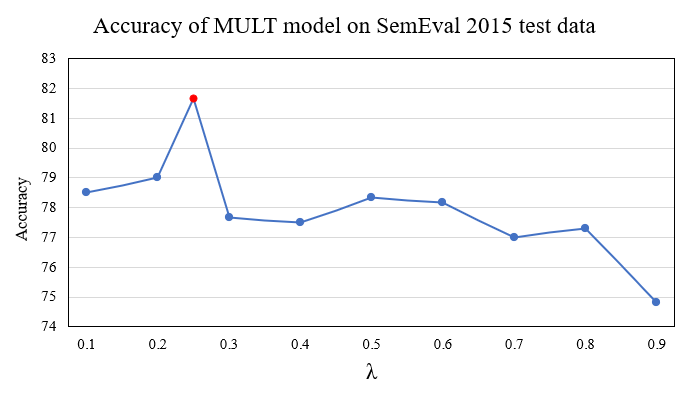
\includegraphics[scale=0.85]{Images/mult.PNG}
    \caption{Accuracy of the MULT model for different sizes of $\lambda$. The red data point is the optimal $\lambda$, at a value of 0.25.}
    \label{fig:multLambda}
\end{figure}




\section{Conclusion}
ABSC models are constrained due to the limited availability of aspect-level training data. In this paper, we try to overcome this limitation by using document-level training data to train the state-of-the-art LCR-Rot-Hop++ model. The results show that the most successful transfer learning approach is multi-task learning, particularly when faced with a small and imbalanced dataset such as SemEval 2015. Likely, multi-task learning outperforms the pretraining approach due to catastrophic forgetting; document knowledge acquired in pretraining is partly forgotten when the model is retrained on aspects. Multi-task learning solves this problem by fitting on the main and auxiliary task simultaneously, preventing this type of forgetting \cite{Chen2020}. 

Our best approach, the MULT model, yields a 2.2 percentage point increase relative to the state-of-the-art LCR-Rot-hop++ model with L1 and L2 regularisation for the SemEval 2015 dataset, as well as a 0.4 percentage point increase for the SemEval 2016 dataset. Furthermore, this model performs equally well as the HAABSA++ model for the SemEval 2015 dataset and better than the HAABSA++ model for the SemEval 2016 dataset. Therefore, we conclude that the inclusion of L1 and L2 regularisation terms along with the MULT method of document knowledge transfer can effectively compensate for the exclusion of an ontology step. Hence, this updated model can serve as a computationally cheaper alternative to existing hybrid models, without any significant loss in performance.

A suggestion for future research is to investigate different deep learning architectures for incorporating document knowledge transfer. One example of a different architecture is adding a shared BiLSTM layer below the LCR-Rot-hop++ model, instead of sharing the left, middle and right BiLSTM. Furthermore, future research can investigate models that exploit sentence or paragraph level knowledge, besides document level knowledge.  
\bibliographystyle{OurArticles/splncs04.bst}
\bibliography{OurArticles/references3.bib}
\section*{Appendix}
\subsection*{A. Hyperparameter optimization}
\renewcommand{\thefigure}{A\arabic{figure}}
\setcounter{figure}{0}
\renewcommand{\thetable}{A\arabic{table}}
\setcounter{table}{0}

In this appendix we provide the optimal values of the hyperparameters for both the FT-based models and the MULT-based models. Thus, Table A1 shows the hyperparameters of the two different categories of models for each dataset. 

\begin{table}[h]
\caption{Optimal hyperparameters of FT-based and MULT-based models based on SemEval 2015 and SemEval 2016.}
\label{tab:hyperparams}
\setlength{\tabcolsep}{24pt}
\begin{tabular}{@{}lcccc@{}}
\toprule
               & \multicolumn{2}{c}{SemEval 2015} & \multicolumn{2}{c}{SemEval 2016} \\ \cmidrule(l){2-5} 
               & FT              & MULT           & FT              & MULT           \\ \midrule
L1 regulariser & $10^{-9}$           & $10^{-7}$          & $10^{-4}$           & $10^{-5}$          \\
L2 regulariser & 0.000           & 0.001          & 0.000           & 0.000          \\
Learning rate  & 0.001           & 0.001          & 0.001           & 0.001          \\
Dropout rate 1 & 0.3             & 0.3            & 0.5             & 0.6            \\
Dropout rate 2 & 0.4             & 0.6            & 0.6             & 0.5            \\
d   & 400             & 250            & 200             & 400            \\
Lambda         &                 & 0.25           &                 & 0.5            \\ \bottomrule
\end{tabular}
\footnotesize\textit{Note}. Dropout rate 1 refers to the dropout rate at the input layer, while dropout rate 2 refers to the dropout rate after the BiLSTM layer.
\end{table}

\subsection*{B. Confusion matrix and sensitivity analysis}
\renewcommand{\thefigure}{B\arabic{figure}}
\setcounter{figure}{0}
\renewcommand{\thetable}{B\arabic{table}}
\setcounter{table}{0}

Table \ref{tab:confusion matrix:pret} shows the confusion matrix of the PRET+FT model on the SemEval 2015 dataset. The behaviour is similar to the MULT model as discussed in Sect. 5.2, however less pronounced and performance-enhancing.
\begin{table}[h!]
\caption{Confusion matrix of the PRET+FT model with document knowledge transfer for the SemEval 2015 data.}
\label{tab:confusion matrix:pret}
\setlength{\tabcolsep}{28.3pt}
\begin{tabular}{@{}lccc@{}}
\toprule
                   & \multicolumn{3}{c}{Predicted sentiment} \\ \midrule
 Observed sentiment & Negative     & Neutral    & Positive    \\ \midrule
 Negative           & 161          & 4          & 43          \\
 Neutral            & 19           & 4          & 15          \\
 Positive           & 35           & 1          & 318         \\ \bottomrule
 \end{tabular}
 \end{table}
 
 Fig. \ref{fig:pret+ft} shows the model performance for PRET+FT on the SemEval 2015 dataset with varying sizes of the pretraining corpus. The size of the pretraining corpus is step-wise enlarged by 3000. Note that for any of the inspected sizes, the performance does not deteriorate with respect to the LCR-Rot-Hop++ benchmark model, which is equivalent to PRET+FT with a pretraining corpus size of 0. This means that adding domain-relevant documents in the PRET stage will likely not harm the model. Up until 12000 documents, the validation accuracy follows an upwards trend. This suggests that some document knowledge transfers well to the aspect level. However, after its peak at 12000, both the accuracy and macro-F1 seem to jitter. This suggests that too much pretraining data is fed into the model, leading to overfitting on the auxiliary task and underfitting on our main task.
 
 \begin{figure}[h!]
    \centering
    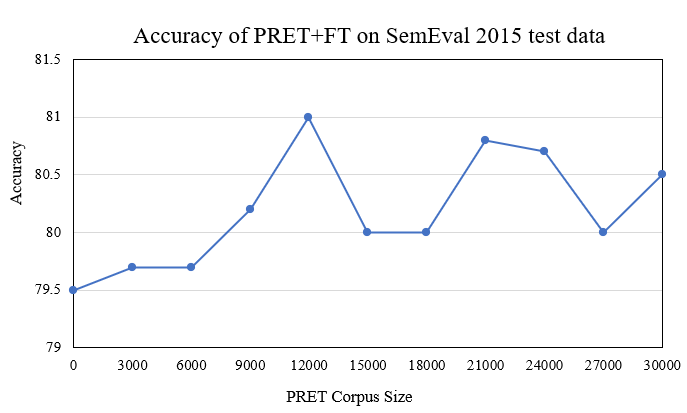
\includegraphics[scale =0.8]{Images/PRET+FT.PNG}
    \caption{Performance of the PRET+FT model for varying pretraining corpus sizes.}
    \label{fig:pret+ft}
\end{figure}
\end{document}
